\chapter{Avaliação}
\label{c_avaliacao}
Essa pesquisa seguiu uma abordagem qualitativa exploratória, e buscou gerar dados descritivos e explanatórios. O objetivo foi descrever as interações das crianças com uma interface de RA projetiva durante a programação e depuração de algoritmos em um ambiente educacional infantil. Além disso, os método buscou captar as percepções de professores a respeito da proposta. Neste sentido, a \autoref{sec:contexto} descreve o contexto de realização da pesquisa, a \autoref{sec:participantes} descreve os participantes, e a \autoref{sec:ambiente} detalha o ambiente escolar. Por fim, a \autoref{sec:protocolo} apresenta os instrumentos de coleta.
 
\section{Contexto}
\label{sec:contexto}
\subsection{Município}\\
A coleta de dados ocorreu em um \ac{CDI} no município de Gaspar, no estado de Santa Catarina. Dados do IBGE (Instituto Brasileiro de Geografia e Estatística) permitem comparar o município em relação ao demais municípios do Brasil\footnote{\url{https://cidades.ibge.gov.br/brasil/sc/gaspar/panorama}}. Em aspectos populacionais, a cidade está entre as 10\% mais populosas do Brasil (70 mil habitantes). É um local com alta disponibilidade de emprego, estando entre as 5\% cidades brasileiras com maior ocupação (41,8\% da população).
 
Quanto à saúde, a cidade tem uma taxa de 9,05 mortes a cada 1000 nascidos vivos, o que a coloca na metade inferior do ranking de municípios do Brasil. Por outro lado, está entre os 10\% de cidades brasileiras com maior cobertura de esgotamento sanitário (87,3\%).
 
Em aspectos educacionais, a taxa de escolarização entre 6 e 14 anos é 93.7%, o que é próximo da média brasileira. Já o desempenho no \ac{IDEB} para anos iniciais é maior que 74\% dos municípios brasileiros, tendo nota 6,3. Essa nota diminui nos anos finais (4,7), tendência que também é acompanhada pelos demais municípios.
 
Em resumo, em relação aos demais municípios, percebe-se que é Gaspar é uma cidade populosa, com condições sanitárias adequadas, escolarização média e desenvolvimento educacional de médio a alto. Certamente esses dados não permitem uma visão completa ou profunda do contexto municipal, mas permitem posicioná-lo em aspectos de população, saúde e educação em relação ao Brasil. A próxima seção aprofunda a descrição do CDI onde se deu a pesquisa.
 
\subsection{Centro de Desenvolvimento Infantil}
\label{sec:cdi}
A pesquisa ocorreu em um \ac{CDI} de um bairro urbano, distante aproximadamente cinco quilômetros do centro da cidade. O local foi selecionado por conveniência, facilitado pelo contato com uma professora que leciona no local, o que possibilitou pesquisas em anos anteriores. A pesquisa atual, entretanto, não ocorreu nas turmas desta professora. Além disso, nenhum dos participantes conhecia o brinquedo RoPE. Outro critério para a seleção do centro foi a presença de internet, dado que o projetor e a Ct Puzzle Platform são acessíveis por conexão sem fio local.
 
O \ac{PPP} do \ac{CDI} apresenta dados históricos e da estrutura física do local. O mesmo foi fundado em 1990, sendo uma parceria entre a prefeitura municipal e a associação de moradores do bairro. Atualmente possui 38 colaboradores, que promovem o atendimento de 246 crianças. A idade atendida vai de zero e cinco anos e onze meses, e há 12 turmas organizadas em três grupos etários: Infância I (0 a 2 anos), Infância II (2 a 4 anos) e Infância III (4 a 6 anos). Dentro de cada grupo etário as turmas também são divididas. Na Infância III, por exemplo, há turmas de 4 a 5 e de 5 a 6 anos. O espaço tem 9 salas onde as professoras realizam suas atividades, uma biblioteca com aproximadamente 300 livros infantis, um parquinho, banheiros, sala de coordenação e sala do zelador. Além das salas existentes, está em curso a construção de novos espaços no local onde antes havia o parquinho, o qual foi deslocado para um espaço ao lado do CDI.
 
O \ac{PPP} do \ac{CDI} apresenta um diagnóstico da comunidade, construído a partir de um questionário. O trabalho apresenta gráficos de pizza, que serão analisados visualmente pois não apresentam dados numéricos (\autoref{fig:contexto_ppp}). Aproximadamente 2/3 das crianças moram com pai e mãe, metade vai de carro ao \ac{CDI}, e quase a metade não tem computador em casa. A respeito dos pais, a maior parte auxilia os filhos nas atividades do \ac{CDI} mas não tem disponibilidade em horário comercial. A renda de aproximadamente a metade das famílias é de 1 a 2 salários-mínimos, e a outra metade vai de 2 a 4.
 
\begin{figure}[!htbp]
   \centering
   \begin{subfigure}{.3\linewidth}
       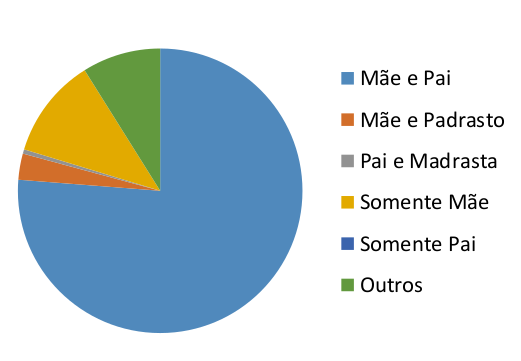
\includegraphics[width=.9\linewidth,fbox]{figs/cdi/mora_com.png}
       \caption{Com quem a criança mora.}
       \label{fig:mora_com}
   \end{subfigure}%
   \begin{subfigure}{.3\textwidth}
       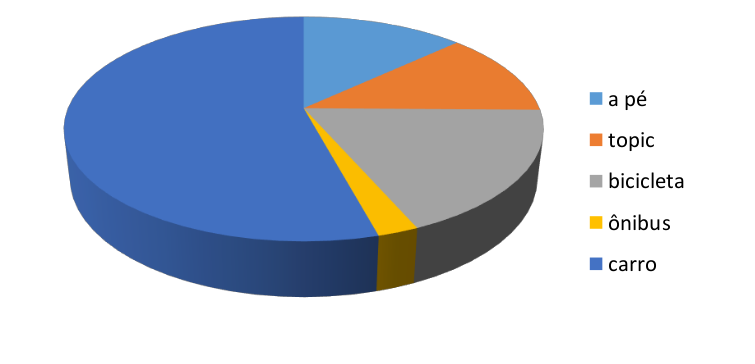
\includegraphics[width=.9\linewidth,fbox]{figs/cdi/meio_transporte.png}
       \caption{Meio de transporte.}
       \label{fig:transporte}
   \end{subfigure}%
  \begin{subfigure}{.3\textwidth}
       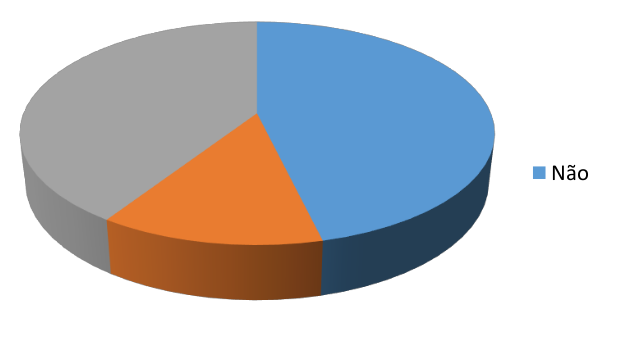
\includegraphics[width=.9\linewidth,fbox]{figs/cdi/tem_computador.png}
       \caption{Tem computador em casa?}
       \label{fig:tem_computador}
   \end{subfigure}
   \begin{subfigure}{.3\textwidth}
       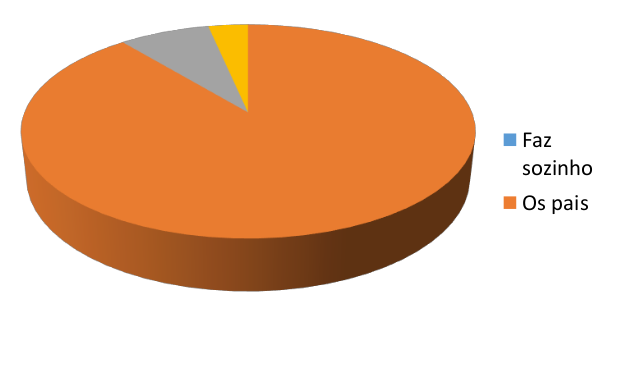
\includegraphics[width=.9\linewidth,fbox]{figs/cdi/pai_auxilia_crianca_atividades.png}
       \caption{Auxílio dos pais nas atividades do CDI}
       \label{fig:pai_auxilia_crianca_atividades}
   \end{subfigure}%
   \begin{subfigure}{.3\textwidth}
       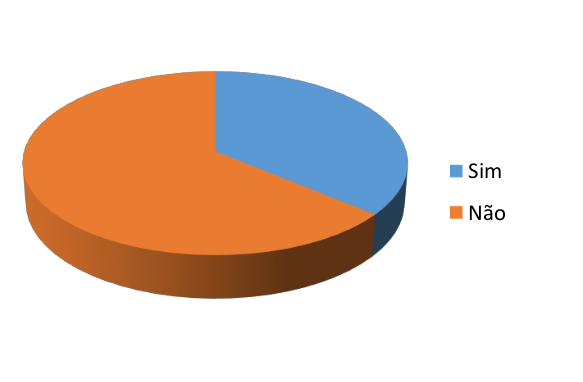
\includegraphics[width=.9\linewidth,fbox]{figs/cdi/disponibilidade_pais_horario_comercial.png}
       \caption{Disponibilidade dos pais em horário comercial.}
       \label{fig:disponibilidade_pais_horario_comercial}
   \end{subfigure}%
    \begin{subfigure}{.3\textwidth}
       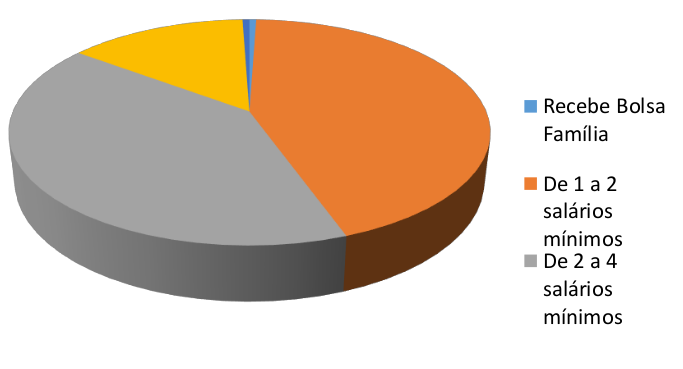
\includegraphics[width=.9\linewidth,fbox]{figs/cdi/renda.png}
       \caption{Renda mensal familiar.}
       \label{fig:renda}
   \end{subfigure}%
   \caption{Dados do Projeto Político Pedagógico do CDI.}
   \label{fig:contexto_ppp}
\end{figure}
Considerando os dados de ocupação da população, providos pelo IBGE, e os gráficos apresentados no \ac{PPP}, infere-se que as condições de vida na região não são precárias, porém a necessidade de trabalho impede o acompanhamento dos filhos em horário comercial. Em horário compatível, porém, os pais buscam auxiliar os filhos nas atividades escolares.
 
\subsection{Proposta Pedagógica para a Educação Infantil}
Mesmo com as suas particularidades locais, todos os CDIs de Gaspar buscam seguir uma mesma proposta pedagógica alinhada com a rede de ensino do municipal. O documento orientador é a Proposta Pedagógica da Rede Municipal para a Educação Infantil \cite{gaspar_proposta_2010}. Essa proposta foi publicada em 2010, após ser construída coletivamente pelos professores e professoras da Rede Municipal de Educação Infantil. O resultado é um documento que busca nortear o trabalho pedagógico “para e com” as crianças pequenas.
 
Este “norte” tem duas bases principais: os eixos de Linguagens, Interações e Brincadeiras, e a abordagem metodológica de projetos. Quanto aos eixos, o eixo de Linguagens tem como objetivo incrementar as aprendizagens infantis por meio de atividades que envolvam uso do corpo (linguagem motora); exploração dos sons (linguagem musical); exploração de cores, formas e texturas (linguagem plástica); fala e códigos (linguagem oral e escrita) e noções de espaço, quantidade e números (linguagem matemática). O eixo de Interações diz respeito ao planejamento e organização de situações de contato entre criança-criança, criança-adulto e criança-objeto. Por fim, o eixo das brincadeiras busca aumentar o repertório de interações lúdicas entre as crianças, orientando o educador a observar, coordenar ou integrar-se nas brincadeiras.
 
Já a Metodologia de Projetos, segundo a proposta, é uma abordagem que permite combinar as intenções pedagógicas do adulto e também estimular a curiosidade da criança. Esse estímulo se dá ao propor projetos em que há investigação de algum tema ou construção de algo com foco em assuntos do mundo infantil (ver \autoref{fig:tres_porquinhos}). Os temas dos projetos surgem em diálogos durante rodas de conversa, passeios ou brincadeiras. Partindo do interesse das crianças, os projetos seguem uma estrutura com hipóteses, perguntas de pesquisa, descrições e comparações. Não há prazo de início e fim, e também não há necessidade de trabalhar diariamente com projetos. Quando nenhum projeto está em curso, trabalha-se seguindo os eixos de Linguagens, Interações e Brincadeiras.
 
\begin{figure}[!h]
   \centering
   \begin{subfigure}{.45\linewidth}
       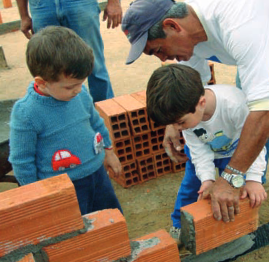
\includegraphics[width=.8\linewidth,fbox]{figs/tres_porquinhos.png}
       \caption{Projeto de construção de casa de tijolos (História dos Três Porquinhos).}
       \source{Proposta Pedagógica da Rede Municipal de Educação Infantil de Gaspar (2010). }
       \label{fig:tres_porquinhos}
   \end{subfigure}%
   \hspace{.05\textwidth}%
   \begin{subfigure}{.45\textwidth}
       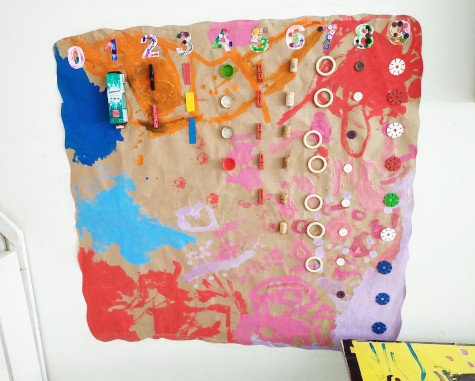
\includegraphics[width=.8\linewidth,fbox]{figs/projeto_numeros_menor.jpeg}
       \caption{Projeto para assimilação de quantidades. Turma de 4 a 5 anos.}
       \source{O autor.}
       \label{fig:projeto_numeros}
   \end{subfigure}%
\end{figure}
A proposta não menciona diretamente o tema das tecnologias digitais. Palavras como \textit{celular} e \textit{computador} não são citadas. Ainda assim, a relação com o “mundo digital” é aderente aos eixos e abordagens metodológicas propostas. As interações, por exemplo, podem ser favorecidas pelo RoPE AR, quando a criança aperta botões e encaixa blocos que provocam reações em um objeto. Há também o uso de uma Linguagem para comunicar uma sequência de ações a um objeto (o brinquedo RoPE). Por fim, a atividade em si é uma Brincadeira, que segundo a proposta deve envolver elementos acolhedores, desafiadores e inclusivos \cite[p.50]{gaspar_proposta_2010}.



% restaurante, canto caverna, castelo das bonecas, área de animais aquáticos, robô

\section{Participantes da pesquisa}
\label{sec:participantes}

Participaram da pesquisa 20 crianças e 3 professoras de um CDI público, além do pesquisador. As crianças tem entre 4 a 6 anos, e frequentam o CDI no período matutino ou vespertino, em semanas alternadas. Quanto às professoras, são mulheres, com formação em Pedagogia e com mais de 10 anos de dedicação à Educação Infantil. Elas declaram ser inábeis para trabalhar com tecnologias digitais "avançadas", mas usam softwares como editores de texto e navegadores de internet para planejar as atividades com as crianças. O pesquisador é um homem de 26 anos, com formação em Ciência da Computação e experiência em desenvolvimento de softwares empresariais.

A participação das professoras e crianças se deu em três salas. A primeira sala atende crianças entre 5 e 6 anos (5-6A), enquanto as outras duas atendem crianças entre 4 e 5 anos (4-5A e 4-5B). Cada sala recebe crianças diferentes no período matutino e vespertino.

No primeiro dia da pesquisa, a atividade ocorreu na sala de 5-6A, durante a tarde. No segundo dia a visita ocorreu na sala 4-5A. Por fim, no terceiro dia, a sala visitada foi a 4-5B, tanto de manhã quanto à tarde. Deste modo, quatro grupos de crianças participaram (\autoref{quadro:participants}):

 \begin{quadro}[!h]
 		\setlength{\extrarowheight}{3pt}
        \begin{center}
        \caption{Encontros e participantes}
        \label{quadro:participants}
        \begin{tabular}{@{}llcccc@{}}
            \toprule
            Grupo & Encontro & Turma                    & Meninas & Meninos & Professoras \\ \midrule
            1     & Dia 1    & 5 a 6 anos - Tarde       & 3       & 2       & Daiana e Maria \\
            2     & Dia 2    & 4 a 5 anos A - Tarde     & 0       & 3       & Paula e Joana \\
            3     & Dia 3    & 4 a 5 anos B - Manhã     & 4       & 2       & Vera e Lúcia \\
            4     & Dia 3    & 4 a 5 anos B - Tarde     & 2       & 4       & Vera e Lúcia \\ \midrule
            4 grupos   & 3 dias & 5 turmas              & 9       & 11      & Seis professoras \\ \bottomrule 
            \end{tabular}
        \end{center}
        \sourceauthor
    \end{quadro}

A distribuição por sexo ficou balanceada, com 9 meninas e 11 meninos. Já a distribuição por idade tendeu a concentrar-se entre 4 e 5 anos (\autoref{fig:ages}), com mediana de 4,58 e média 4,71. Isso é compreensível pois os experimentos ocorreram em duas salas com crianças de 4 a 5 anos e em apenas uma sala com crianças de 5 a 6 anos.

\begin{figure}[!htpb]
    \centering
    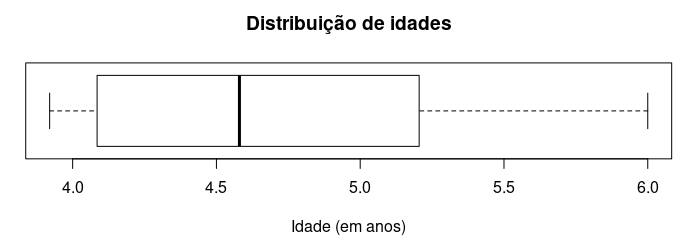
\includegraphics[width=.6\linewidth,fbox]{figs/ages.png}
    \caption{Distribuição de idades.}
    \sourceauthor
    \label{fig:ages}
\end{figure}

Cada sala possui uma professora e uma assistente, denominadas aqui de professoras. Todas são mulheres, e possuem de 4 a 28 anos de experiência de trabalho com crianças. Das seis professoras participantes, três responderam diretamente a entrevistas e outras três colaboraram em algum momento por meio de comentários a respeito do projeto ou auxiliando na comunicação com as crianças. Os nomes utilizados no texto são fictícios, a fim de evitar a identificação dos participantes
 
O recrutamento, portanto, se deu por conveniência. As crianças participantes frequentavam o ambiente no dia da visita do pesquisador. Não houve distinção de sexo ou presença/ausência de deficiência intelectual. A ordem de participação das crianças se deu com o pesquisador solicitando a participação de crianças e as professoras selecionando as mesmas. As crianças que quiseram participar antes da solicitação não foram impedidas. Deste modo, não houve um controle rígido do acesso à interface, mas sim uma organização para evitar mais de três crianças utilizando ao mesmo tempo. Quanto às professoras, participaram das entrevistas as responsáveis pela turma em questão ou as que se sentiram confortáveis em responder.

\section{Ambiente}
\label{sec:ambiente}
As atividades ocorreram em três salas comumente frequentadas pelas crianças. Em todas as salas o projetor ficou em um suporte, posicionado ao lado de uma fonte de energia e afastado de janelas e portas. As luzes das salas foram apagadas, mas isso não modificou o ambiente a ponto de torná-lo escuro (ver \autoref{fig:setting}). No chão, à frente do projetor, foram fixadas duas cartolinas brancas para receber as imagens projetadas. Ao lado do projetor um notebook foi posicionado para servir como câmera. 

\begin{figure}[!h]
    \centering
    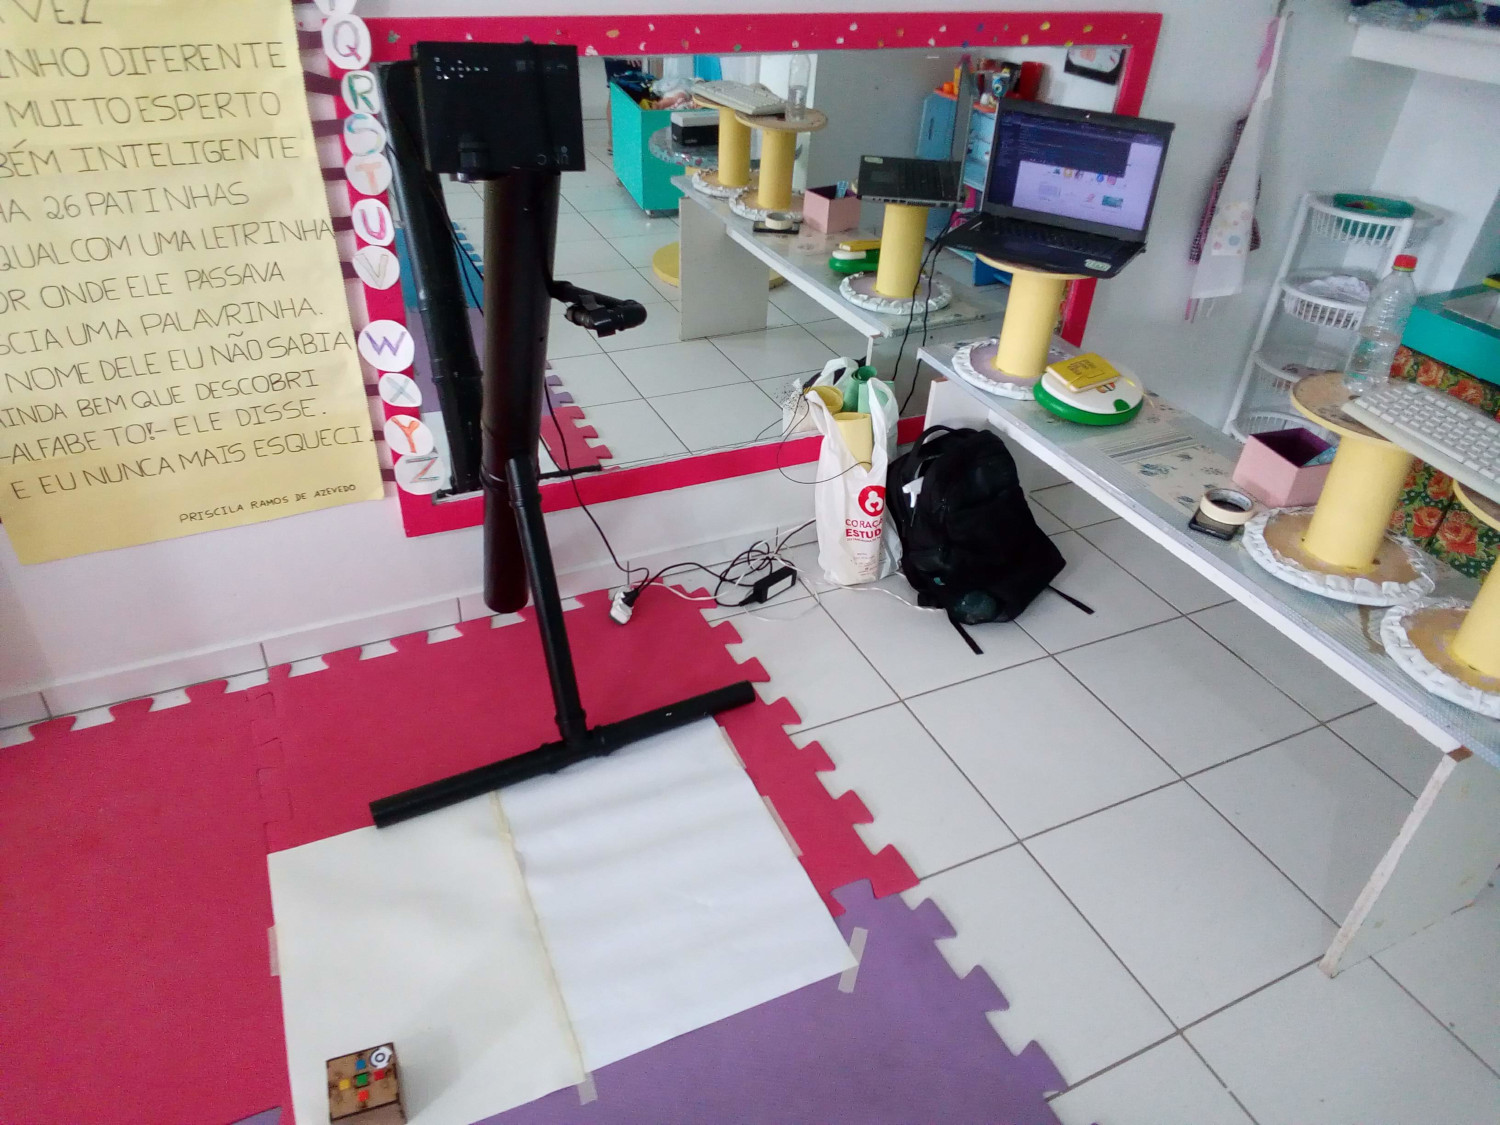
\includegraphics[width=0.8\textwidth,fbox]{figs/setting_projector.jpg}
    \caption{Posicionamento do projetor.}
    \label{fig:setting}
\end{figure}

As crianças continuaram suas atividades junto às professoras enquanto o pesquisador organizava os equipamentos. Era perceptível a curiosidade a respeito dos materiais e da figura do pesquisador, tanto pelos olhares quanto por perguntas feitas às professoras. Ao lado da sala da turma 4-5A há um espaço externo gramado. Neste ambiente a professora continuou as atividades no espaço externo, e a programação do RoPE ocorreu dentro da sala com a outra professora presente. As outras duas salas tem espaços amplos, e todas as crianças permaneceram no ambiente durante a atividade. Enquanto duas ou três crianças participavam da pesquisa, as demais continuavam suas atividades em outro ponto da sala.
 
O CDI tem rede de internet sem fio, porém a qualidade do sinal é variável em diferentes salas. Especificamente a sala 4-5A apresenta problema de quedas constantes de conexão. Esse problema foi mencionado pelas professoras e ocorreu durante a conexão do projetor na rede local. As demais salas visitadas, porém, tem conexão estável.

\section{Coleta de Dados}
\label{sec:protocolo}
A coleta de dados gerou três artefatos: vídeos das interações de crianças com a RoPE AR, entrevistas com as professoras que acompanharam essas interações, e a lista dos algoritmos criados pelas crianças, registrados na CtPuzzle Platform. 

\subsection{Vídeos de interações}
A gravação das interações ocorreu logo após a organização do ambiente. Foram gravadas interações de crianças, as quais trabalharam em duplas, trios ou individualmente, solucionando desafios de programação e depuração. Um protocolo definiu as etapas e os materiais\footnote{
    Materiais utilizados:
    \begin{itemize}
        \item Projetor (UC46)
        \item RoPE
        \item Smartphone Android (Modelos testados: M5c e Redmi 8)
        \item Duas cartolinas brancas (coladas no chão, receberam a imagem projetada)
        \item Suporte para o projetor
        \item Blocos de papelão
        \item Folha de consentimento
        \item Conexão com a internet
        \item Notebook (webcam para gravação dos vídeos)
    \end{itemize}
} a serem usados durante essas interações. Apesar de definir a sequência de ações, o protocolo não impediu flexibilizá-las, de modo a se adaptarem às sugestões das crianças, dificuldades, curiosidades, e restrições de tempo existentes.

\begin{enumerate}
    \item Seleção: a seleção das crianças participantes em cada atividade se deu com o pesquisador na sala de aula, perguntando quais crianças gostariam de iniciar a participação na atividade. As professoras então selecionaram as crianças, em grupos de 2 ou 3, escolhendo as que estavam mais próximas umas das outras. Na sala 3 houve alternância de crianças entre os grupos, de modo que crianças entraram e saíram durante a atividade, mas procurando manter um número máximo de 3 crianças simultâneas. Na sala 2 as professoras selecionaram as crianças que consideram ter mais e menos dificuldades de compreensão.
    
    \item Ambientação: a ambientação ocorreu como uma conversa inicial entre pesquisador e as crianças, sentados em tapetes emborrachados, próximos ao projetor. O pesquisador perguntou se elas conheciam algum robô. Elas então responderam com frases como \fala{o meu robô sai luzes}, ou \fala{eu lembro daquele robô daquele filme}. Após isso, as crianças foram instigadas a descrever a aparência e as ações do robô. Por fim, o pesquisador apresentou o RoPE, e falou que ele seria “programado” usando os bloquinhos de papelão.
    
    \item Reconhecimento dos blocos: para cada um dos cinco blocos, em ordem aleatória, as crianças responderam a pergunta \fala{o que vocês acham que ele [o robô] está fazendo neste desenho aqui?}. A intenção foi ouvir as respostas, sem julgamentos. Em caso de respostas como \fala{ele está olhando pro lado}, o pesquisador perguntou pra que lado ele estava \fala{olhando}\footnote{Nos desenhos que representam o robô \destaque{girando}.}. Os blocos ficaram ao alcance das crianças, e se observou como as mesmas os manipulavam e se identificavam alguma relação com os botões do RoPE. Buscou-se permitir liberdade durante essas interações: em certa ocasião, por ter blocos repetidos, as crianças acharam que os mesmos representavam um jogo da memória, o qual foi imediatamente jogado.
    
    \item Programação: o aplicativo e a projeção foram ligados, e as crianças descreveram o que viam na área projetada. O pesquisador explicou às crianças que a tarefa consistia em ajudar o RoPE andar pelo caminho marrom e pegar a maçã, e para isso deveriam usar os blocos. Para a primeira maçã, o pesquisador explicou o funcionamento, colocando o RoPE na posição inicial, encaixando o bloco Frente no bloco Início e apertando o botão Iniciar do RoPE. As crianças então usaram os blocos e programaram o robô para coletar as próximas quatro maçãs (\autoref{quadro:fases_programacao}).
    
    A complexidade da solução de cada uma das fases apresentadas é crescente. Enquanto a primeira fase exige apenas um comando, a segunda exige dois. A terceira fase também exige dois comandos, porém acrescenta o comando de giro. Além do maior número de comandos, a orientação da criança em relação ao RoPE é outro fator que dificulta a resolução. Nas fases 1 e 2 a criança programa o robô estando na mesma orientação que ele. Nas fases 3 a 5, porém, o robô está com seu lado direito voltado para a criança, e portanto ela precisa imaginar-se em outra perspectiva ou se mover para a mesma orientação que o brinquedo\footnote{Piaget e Inhelder (1981) citam a dificuldade que crianças têm de imaginar-se em outra perspectiva (egocentrismo).}.
    
    Dúvidas e erros surgiram com frequência durante a programação, e o pesquisador auxiliou fazendo perguntas e dando exemplos quando necessário, e explicando as regras e direções.
    
    \item Depuração: Nesta etapa as crianças foram questionadas a encontrar erros em um algoritmo criado pelo pesquisador. Por quatro vezes, este sequenciou blocos de modo que o brinquedo não coletasse a maçã (\autoref{quadro:fases_depuracao}). Se, apenas observando a sequência, as crianças não encontraram o erro, o pesquisador solicitou para apertarem o botão Iniciar para ver o robô andar de modo incorreto. As crianças então editaram a sequência de blocos. Nos casos em que a edição do programa ainda não corrigiu o erro, o pesquisador reposicionou o brinquedo no ponto inicial. Enquanto o objetivo da etapa de programação foi a criança \destaque{construir} algoritmos, a intenção da fase de depuração foi favorecer a \destaque{avaliação} do algoritmo, de modo que que as crianças pudessem olhar, discutir, modificar e testar o programa para eliminar o bug e resolver o problema.

\end{enumerate}

\begin{quadro}[htbp]
    \captionquadro{Fases de programação}
    \label{quadro:fases_programacao}
    \begin{longtable}{ | m{.2\textwidth} | m{.5\textwidth} | m{.2\textwidth} | }
        \hline
        \textbf{Fase}  & \textbf{Descrição} & \textbf{Solução esperada} \\ \hline
        \endhead
        
        %%%%%%%%%%%%%%%%%%%
    
        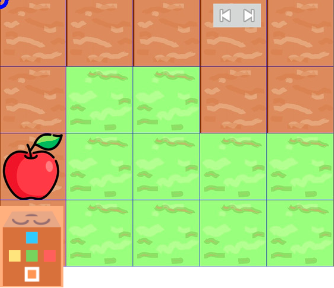
\includegraphics[width=.9\linewidth]{figs/prog/1.png} &
    
        \textbf{Fase 1}: 
        Primeira fase e a mais simples. O desafio é andar apenas um passo à frente. A intenção é que a criança compreenda que o robo se move em correspondência ao bloco encaixado, e que o início da execução ocorre ao apertar o botão verde do robô. &
        
        Frente

        \\ \hline
    
        %%%%%%%%%%%%%%%%%%%
    
        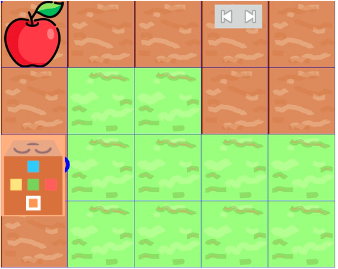
\includegraphics[width=.9\linewidth]{figs/prog/2.png} &
    
        \textbf{Fase 2}: 
        A ideia aqui é que a criança compreenda que o robô faz mais de um passo por vez. Precisa justapor dois blocos frente para alcançar o objetivo. & 
        
        Frente, frente

        \\ \hline
    
        %%%%%%%%%%%%%%%%%%%
    
        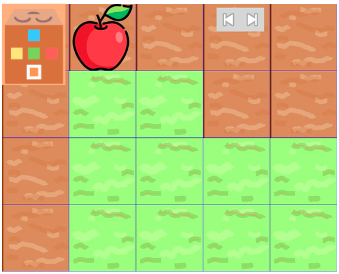
\includegraphics[width=.9\linewidth]{figs/prog/3.png} &
    
        \textbf{Fase 3}: 
        Nesta fase é adicionada o movimento de giro. A maçã aparece do lado direito do robô, que está virado para frente. &

        Direita, frente
        
        \\ \hline
    
        %%%%%%%%%%%%%%%%%%%
    
        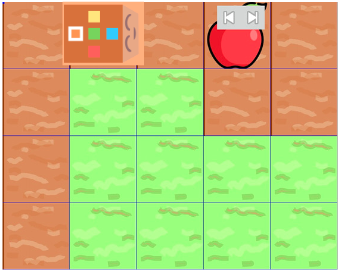
\includegraphics[width=.9\linewidth]{figs/prog/4.png} &
    
        \textbf{Fase 4}:
        A solução desta fase emprega os mesmos comandos que a Fase 2. A diferença é a orientação provável do robô em relação à criança. Se a criança estiver na frente da área projetada, então verá a lateral direita do RoPE. Na Fase 2 criança e robô estão em orientações iguais. &

        Frente, frente
        
        \\ \hline
    
        %%%%%%%%%%%%%%%%%%%
    
        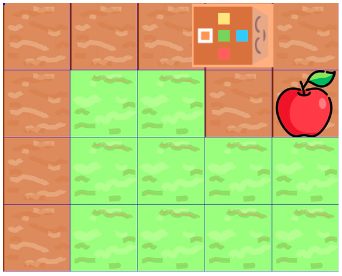
\includegraphics[width=.9\linewidth]{figs/prog/5.png} &
    
        \textbf{Fase 5}: 
        Esta é a fase de programação que exige maior número de comandos (três). Além disso a criança precisa imaginar a posição do robô após o giro, para então decidir o comando a ser usado em seguida (frente).
        &
        Frente, esquerda, frente 
        
        \\ \hline
        
    \end{longtable}
\end{quadro}

\begin{quadro}[htbp]
    \captionquadro{Fases de depuração}
    \label{quadro:fases_depuracao}
    \begin{longtable}{ | m{.2\textwidth} | m{.5\textwidth} | m{.1\textwidth} | m{.1\textwidth} |}
        \hline
        \textbf{Fase}  & \textbf{Descrição} & \textbf{Solução esperada} & \textbf{Tipo de erro} \\ \hline
        \endhead
        
        %%%%%%%%%%%%%%%%%%%
    
         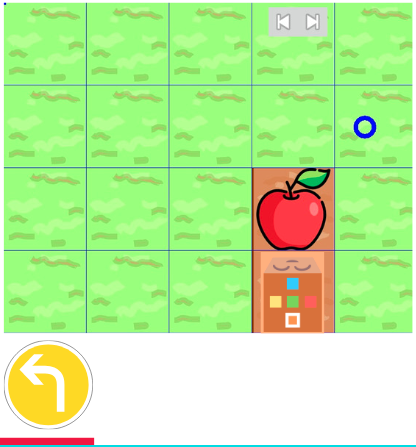
\includegraphics[width=.9\linewidth]{figs/debug/1.png} &
    
         \textbf{Fase 6}: 
         A maçã está logo à frente, porém o algoritmo tem um giro à esquerda. & 
         
         Frente & Comando incorreto
 
         \\ \hline
     
         %%%%%%%%%%%%%%%%%%%
     
         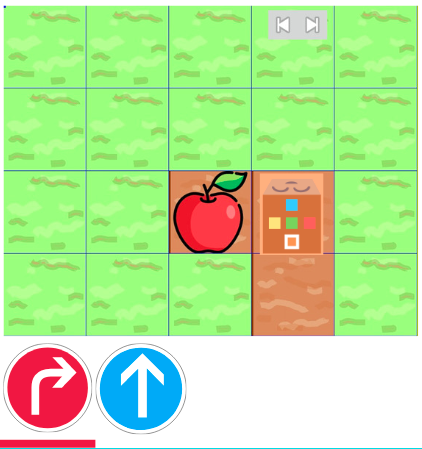
\includegraphics[width=.9\linewidth]{figs/debug/2.png} &
     
         \textbf{Fase 7}: 
         Nesta fase o erro é o comando de giro. O robô precisa girar à esquerda, mas o comando utilizado é o de girar à direita. &
 
         Esquerda, frente & Comando incorreto
         
         \\ \hline
     
         %%%%%%%%%%%%%%%%%%%
     
         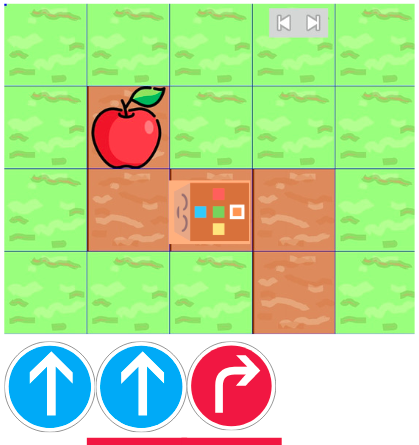
\includegraphics[width=.9\linewidth]{figs/debug/3.png} &
     
         \textbf{Fase 8}:
         O erro nesta fase está na ordem dos comandos utilizados. Se o brinquedo avança duas vezes ele passa da posição onde deve girar à direita. A tarefa consiste em reordenar os comandos já existentes, em vez de adicionar ou remover comandos. &
 
         Frente, direita, frente & Ordem dos comandos
         
         \\ \hline
     
         %%%%%%%%%%%%%%%%%%%
     
         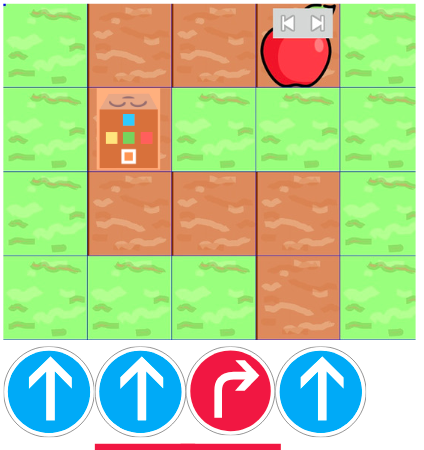
\includegraphics[width=.9\linewidth]{figs/debug/4.png} &
     
         \textbf{Fase 9}: 
         Tarefa de maior dificuldade em todas as etapas, pois exige quatro comandos. Assim como na fase 8, o erro está na ordem dos comandos utilizados.
         &
         Frente, direita, frente, frente & Ordem dos comandos
         
         \\ \hline
     
         %%%%%%%%%%%%%%%%%%%

    \end{longtable}
\end{quadro}

Nas situações em que todas as fases foram concluídas, ou se percebeu que a criança perdeu o interesse na atividade, ou ao final do tempo disponível, o pesquisador agradeceu às crianças, e perguntou se o vídeo da atividade poderia ser usado no seu trabalho. Para isso apresentou uma folha pequena, contendo um rosto alegre e um triste. As crianças então pintaram um dos dois rostos como forma de consentimento. Vale ressaltar que tanto na etapa de programação quanto de depuração, não foi exigida a finalização de todas as fases. Pesquisador e professora decidiram interromper as atividades em casos onde as crianças apresentaram sinais de cansaço ou perderam atenção à tarefa.

Além de não ser exigida a finalização das tarefas, as trajetórias de cada fase serviram como uma sugestão, e não como uma restrição. Ocorreram modificações em que a criança sugeriu um outro ponto de partida ou um caminho mais longo. O aceite ou não destas modificações foi negociado, a fim de haver tentativas nos caminhos pré-definidos e também nos caminhos sugeridos pela criança. Da mesma forma, foi permitida a resolução do problema em etapas, quando a criança programou o brinquedo para andar até metade do caminho, por exemplo, e depois programou os demais passos.

\subsection{Entrevistas com as professoras}
As entrevistas com as professoras ocorreu individualmente, após as atividades com as crianças. O local da entrevista foi o ambiente escolar, enquanto as crianças prosseguiam com outras atividades, acompanhadas por outra professora. 

A entrevista ocorreu de forma semi-estruturada \cite{boni_aprendendo_entrevistar_2005}, com cinco questões abertas previamente definidas (\autoref{quadro:perguntas}). O objetivo das perguntas foi explorar o contexto de trabalho do professor, sua visão a respeito da relação entre crianças e tecnologias digitais, e por fim explorar sua visão sobre a atividade proposta com a RoPE AR. Com consentimento das professoras, os áudios das entrevistas foram gravados e posteriormente transcritos (\autoref{apendice_transcricoes}).

\begin{quadro}[!h]
    \captionquadro{Questionário com as professoras}
    \label{quadro:perguntas}
    {{\renewcommand{\arraystretch}{1.5}
    \begin{longtable}{| m{.5\linewidth} | m{.5\linewidth}| }
        \hline
        Pergunta & Motivação \\ \hline
        \pergunta{Você poderia falar sobre suas experiências e seu dia a dia do seu trabalho voltado à Educação Infantil?} & Compreender as experiências passadas e o contexto de trabalho da professora. \\ \hline

        \pergunta{O que você pensa sobre o contato de crianças com tecnologias digitais?} & Identificar sentimentos do professor em relação à tecnologia e também identificar os dispositivos citados. \\ \hline        

        \pergunta{Que importância você daria para a \destaque{visibilidade} no aprendizado das crianças?} & Verificar se a opinião das professoras se alinha com a proposta da interface. \\ \hline

        \pergunta{Você poderia pensar em alguma atividade usando os mesmos princípios propostos na atividade de hoje, seguindo a ideia de projetar imagens no chão e ter essa interação com um robô?} & Compreender a percepção do professor sobre a aplicabilidade da proposta. \\ \hline

        \pergunta{Que tipos de problemas você percebe na proposta? Quais aspectos poderiam melhorar? } & Identificar falhas da interface na visão do professor. \\ \hline

    \end{longtable}
    }
\end{quadro}

\subsection{Registro de respostas na CtPuzzle Platform}
Como descrito na seção \autoref{sec:ctpuzzle}, a CtPuzzle Platform é uma plataforma que possibilita configurar mecânicas de puzzles com o objetivo de criar testes para avaliação do \ac{PC}. A RoPE AR representa uma mecânica em que há um mapa, um ponto inicial, e um caminho a ser percorrido.

\begin{figure}[!htpb]
    \centering
    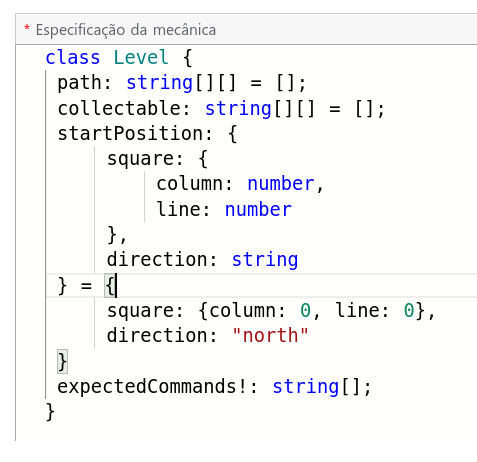
\includegraphics[width=.5\linewidth,fbox]{figs/mecanica.png}
    \caption{Especificação da mecânica.}
    \sourceauthor
    \label{fig:mecanica}
\end{figure}

Após definir os atributos da mecânica (a estrutura que representa as fases do jogo, itens do teste, etc) a plataforma possibilita configurar itens com estes atributos. Estes itens são agrupados em testes. As fases de programação e depuração (\autoref{quadro:fases_programacao} e \autoref{quadro:fases_depuracao}) compõem um teste de 9 itens.

Por fim, cada item tem uma \destaque{resposta esperada}. No caso da RoPE AR, a resposta esperada, para cada fase, é formada por uma sequência de comandos correspondentes a movimentos que o RoPE precisa fazer para alcançar o objetivo. Para cada um dos 9 itens, a comparação entre a resposta esperada e a \destaque{resposta dada} produz um \destaque{escore}. Ele representa a assertividade na solução do problema. Essa comparação se dá numa função de cálculo de escore. A \autoref{fig:item_configurado} mostra a fase 1 configurada na plataforma e instanciada pela RoPE AR: a resposta esperada é um avanço à frente.

\begin{figure}[!htpb]
    \centering
    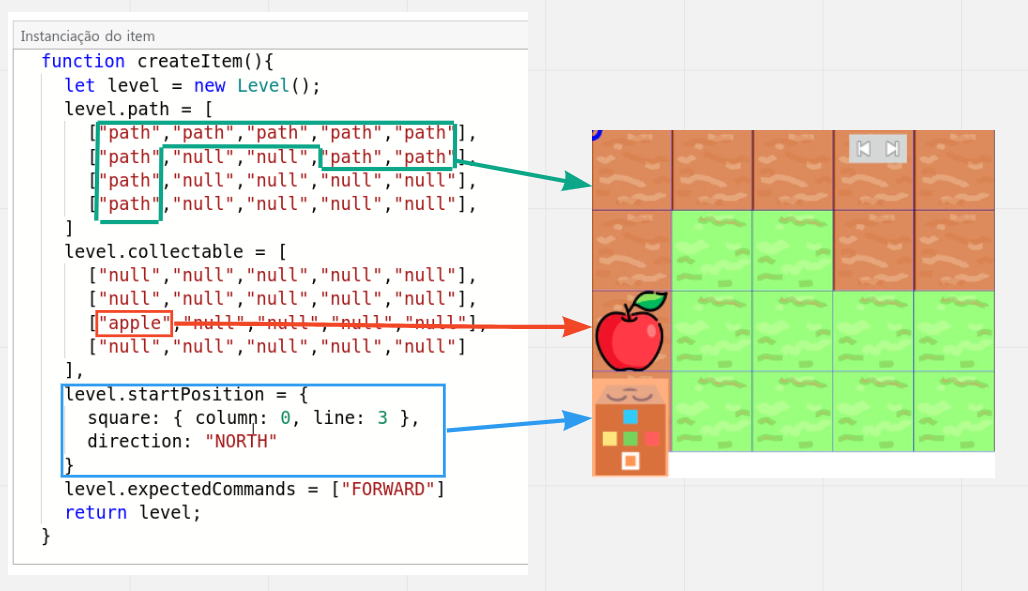
\includegraphics[width=.6\linewidth,fbox]{figs/item_configurado.png}
    \caption{Item configurado na plataforma e instanciado no aplicativo RoPE AR.}
    \sourceauthor
    \label{fig:item_configurado}
\end{figure}

Ressalta-se que, durante a resolução do desafio, é comum a criança realizar mais que uma tentativa. Em cada tentativa ela insere os comandos e pressiona o botão iniciar. A cada início de execução a lista de comandos é armazenada em uma lista de tentativas. Essa lista de comandos usados nas tentativas é utilizada no cálculo do escore.

\section{Análise dos dados}

O processo de análise dos vídeos ocorreu de modos: indutivo e dedutivo. Na análise indutiva os vídeos foram assistidos repetidas vezes, sem uma definição antecipada de códigos\footnote{O Qualcoder, um software do tipo \acro{CAQDAS}, gratuito e de código aberto, serviu como ferramenta de codificação.}. Foram marcados trechos nos quais as crianças transitaram de estados de repouso para estados ativos, considerando suas gesticulações e falas. No decorrer dos vídeos surgiram novos códigos, conforme o olhar do pesquisador se voltou para aspectos que surgiram em cada filmagem. A partir do terceiro vídeo (\autoref{fig:codificacao}), por exemplo, aparecem trechos marcados em amarelo que são códigos ligados a "mediações de um adulto", pois neste caso as professoras interagiram diretamente durante a brincadeira.

\begin{figure}[!htpb]
    \centering
    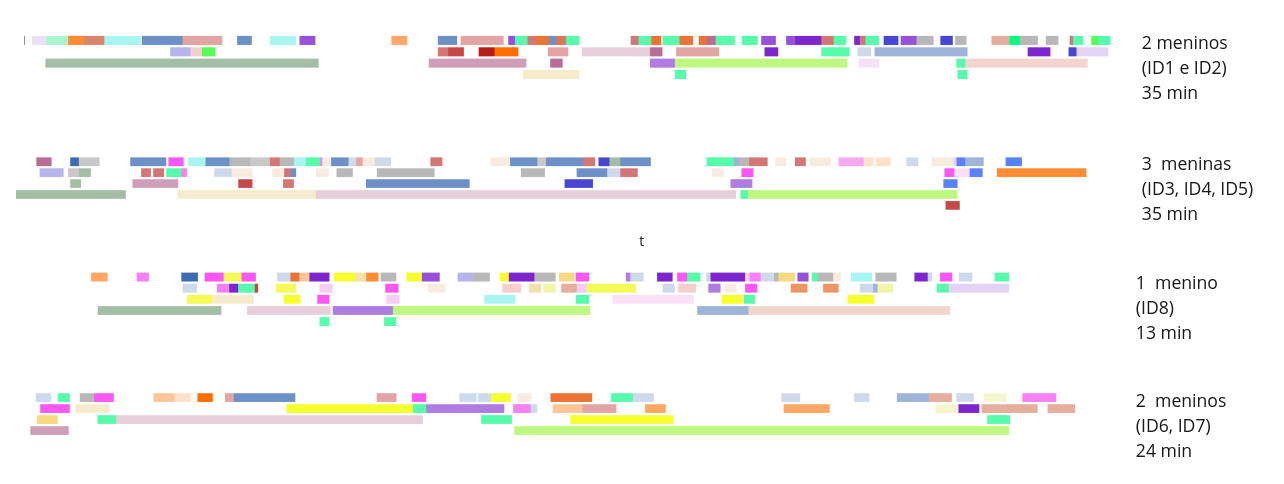
\includegraphics[width=1\linewidth,fbox]{figs/codificacao_aberta.png}
    \caption{Marcações de trechos dos vídeos em cores que indicam seu código.}
    \sourceauthor
    \label{fig:codificacao}
\end{figure}

Esse processo de "codificação aberta"\ permitiu identificar códigos e organizá-los em categorias. As categorias identificadas foram \destaque{Interação com os botões}, \destaque{Interação com os blocos}, \destaque{Interação entre crianças}, \destaque{Depuração}, \destaque{Estratégias de solução de problema}, \destaque{Percepção de realidade aumentada} e \destaque{Mediações de um adulto}. Como foco do trabalho, foram analisadas as categorias relacionadas a interação com os blocos, realidade aumentada e depuração. 

\begin{figure}[!htpb]
    \centering
    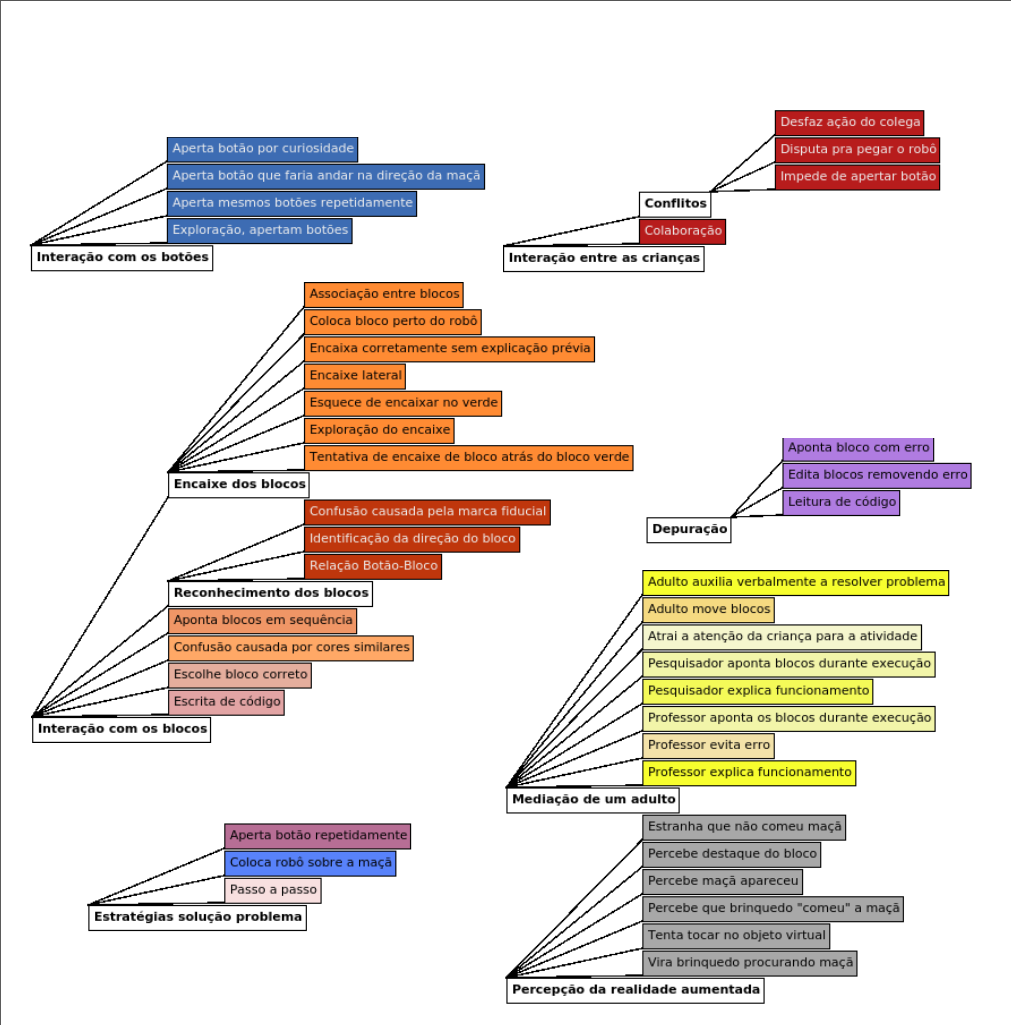
\includegraphics[width=1\linewidth,fbox]{figs/categorias.png}
    \caption{Categorização dos códigos.}
    \sourceauthor
    \label{fig:codificacao}
\end{figure}

A análise dedutiva tem como base o método de análise das filmagens seguido por \citeonline{santana_alise_2015} e \citeonline{blikstein_analyzing_2014}. Esses autores analisam vídeos em que estudantes resolvem desafios de montagem de artefatos físicos, como um brinquedo programável ou uma estrutura em palitos. Nestes trabalhos as ações dos estudantes são codificadas de acordo com uma máquina de estados, em que os estudantes podem estar no estados como Modificar, Planejar, Executar, Refazer e Repousar. Esta pesquisa se apoia no mesmo método por entender que a atividade proposta às crianças envolve a mesma combinação de manipulações físicas e raciocínio lógico voltado à resolução de um problema.

\section{Considerações}

Este capítulo apresentou o ambiente, os participantes, e a coleta de dados da interação com uma interface tangível de programação em blocos, associada a realidade aumentada projetiva. Em resumo, os dados obtidos são vídeos, entrevistas e registros de log, obtidos durante três visitas a um centro de desenvolvimento infantil. O número de participações não é significativo numericamente\footnote{Participação direta de 20 crianças e 3 professoras.}, mas a gravação de vídeos totalizou 4,5 horas de dados passíveis de análise qualitativa, descrita no próximo capítulo.